
\let\oldquote\quote
\let\endoldquote\endquote
\renewenvironment{quote}[2][]
  {\if\relax\detokenize{#1}\relax
     \def\quoteauthor{#2}%
   \else
     \def\quoteauthor{#2~---~#1}%
   \fi
   \oldquote}
  {\par\nobreak\smallskip\hfill(\quoteauthor)%
   \endoldquote\addvspace{\bigskipamount}}


\chapter{Introduction}

%\vspace{-1em}
\begin{quote}{William Shakespeare, \textit{The Tempest}}
    %\noindent 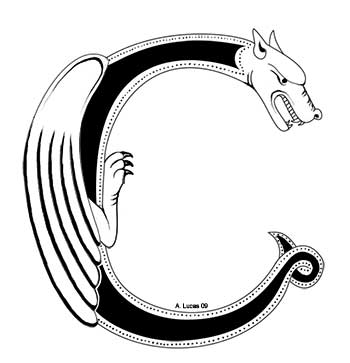
\includegraphics[width=5mm]{ch1/images/finalc.jpg}\textsc{aliban} \\
    \textsc{Caliban} \\
You taught me language, and my profit on ’t \\
Is I know how to curse. The red plague rid you  \\
For learning me your language! (I.ii.362--364)
\end{quote}



The last decade has witnessed an explosion in the expressive capacity of 
\machinelearning~models to generate or manipulate 
%(e.g., paraphrase, simplify, or compress) 
natural language text. In particular, 
\deeplearning-based language models have dramatically improved the overall 
quality of generated text, opening the doors to many exciting applications like
creative writing tools \cite{something} and interactive fiction 
\cite{thatgame}. 
While these new \naturallanguagegeneration~methods are quite powerful, 
they are in practice very difficult to control or constrain. This 
is unfortunate as it limits responsible application to domains with high 
fault tolerance like the those mentioned above and other essentially low stakes,
human guided creative exploration tools. It is unclear if such tools are 
ready for real deployments in domains like crisis informatics \cite{ci}
or medical research aids \cite{something}.

This thesis is focused on a particular \texttotext~generation problem, 
automatic summarization, where the goal is to map a large input text to
a much shorter summary text, and the research presented aims
to ``tame'' these loquacious 
yet mercurial \machinelearning~d{\ae}mons and hopefully pave the way for 
more reliable \texttotext~generation algorithms. 
Somewhat against the prevailing trends, we eschew end-to-end training 
of an abstractive summarization model, and instead breakdown the text 
summarizaion problem into its consituent tasks. 
At a high level, we divide these tasks into two
categories: \contentselection, or ``what to say'' and 
\surfacerealization, or ``how to say it.'' 
Within these categories we propose models or learning algorithms
for the following problems:

\begin{itemize}
    \item Content Selection
        \begin{itemize}
            \item Salience Estimation with \DeepLearning~models
            \item Salience-aware Structured Content Selection models
        \end{itemize}
    \item Surface Realization
        \begin{itemize}
            \item Data Augmentation for Faithful Generation
            \item Linearization Strategies for Content Planning and Controllable Generation
        \end{itemize}
    \end{itemize}


The first part, \contentselection, explores various issues around \salienceestimation, that is,
predicting the importance of an arbitrary unit of text given some surrounding context 
(e.g., the larger document that contains that text or a user query). In 
particular, we experiment with a variety of popular and novel 
\deeplearning~models for salience estimation, and design several ablation
exeriments to gain some insight into the important input signals for making 
predictions. Understanding these signals is critical for designing reliable
summarization models. We then look at two approaches 
for incorporating salience
estimates into larger text extraction algorithms that also consider redundancy
and previous extraction decisions. 

In part two, \surfacerealization, we assume content selection has 
already been performed and focus on methods for \faithfulgeneration, that is,
ensuring that output text utterances respect the semantics of the input
content. While \deeplearning-based \sequencetosequence~models are a popular
model for this problem since they can generate very fluent text, they often
omit, misconstrue, or otherwise generate text that is not semantically
correct given the input content. In this section, we develop a data augmentation technique to aleviate this problem. Additionally, we propose a method
for making a \sequencetosequence~model capable of following a content plan,
allowing for more control over the output utterance generated by the model.


%In this chapter, we develop training strategies for \faithful~and \controllablegeneration~
It is important to note that the approaches in part two are implemented
for solving \taskorienteddialoguegeneration, where
the problem is one of modeling the response of a dialogue agent interacting
with a human user. The input \meaningrepresentation~represents a communicative
goal that the dialogue agent is trying to achieve. While this is technically
a\datatotext~and not a \texttotext~generation problem, the aims
of \faithful~and \controllablegeneration~are relevant to both classes of 
problem
With \datatotext~generation, however, we
get an explicit representation of meaning that makes it easier to make 
experimental progress. We therefore consider 
\taskorienteddialoguegeneration as an idealized form of \texttotext generation,
where content selection has mapped input text units to a 
\meaningrepresentation~of the content to be realized.
Possible ways of bridgeing this gap will be discussed in \autoref{futurework}.

In the remainder of this chapter we briefly give some historical context
for the field \naturallanguagegeneration. 
We then introduce the main contributions of the thesis in more detail
before diving into main the chapters on content selection and surface 
realization. 



%can be thought of 
%as bipartite modules consisting of encoder, which learns to represent and decoder are quite capable
%of generating fluent text, but there is a fundamental tension between the
%
%\deeplearning~based conditional language models produce output text utterances
%that do not semantic
%
%
%
%
%
%In the interest of developing more reliable \machinelearning~models for 
%\texttotext~generation problems, particularly 
%text summarization where a large input text is mapped to a smaller output
%summary text, we eschew the 
%
%
%\texttotext~generation, this papepr 
%
%
%In this work we study several popular models, and propose some of our own,
%for both \texttotext~and \datatotext~generation problems, with the 
%aim of designing experiments to give insight into what signals present in
%the data are actually being used for making predictions, and where possible,
%provide mechanisms or training strategies for control and systematic behavior. 
%
%
%
%Since  `
%
%
%
%
%In this work we explore two modalities of NLG, \texttotext and \datatotext 
%generation.
%
%
%In this work, we 
%explore two applied \naturallanguagegeneration settings, text-to-text and data-to-text
%
%
%
%Natural language generation (NLG) is a subfield of artificial 
%intelligence and computational linguistics broadly interested in algorithms
%for generating natural language text and speech \citep{reiter2000building},
%where the natural languages constitute those naturally arising in 
%human-to-human communication and contrasted with formal languages like LISP, Prolog, or Python \citep{}.
%This thesis makes contributions to two areas of NLG, 
%text summarization and data-to-text generation, using machine learning
%models, and especially deep learning or deep neural network models. 
%
%Machine learning models on natural language data
%can be inscrutable and unpredictable d{\ae}mons, especially as their complexity
%grows. One of the main goals of this work is to understand how
%such models make their decisions, what their limitations are, and how they
%may be used in a more controlled manner. Before further 
%developing our contributions, we begin with some historical context.
%
\begin{figure}
    \centering


    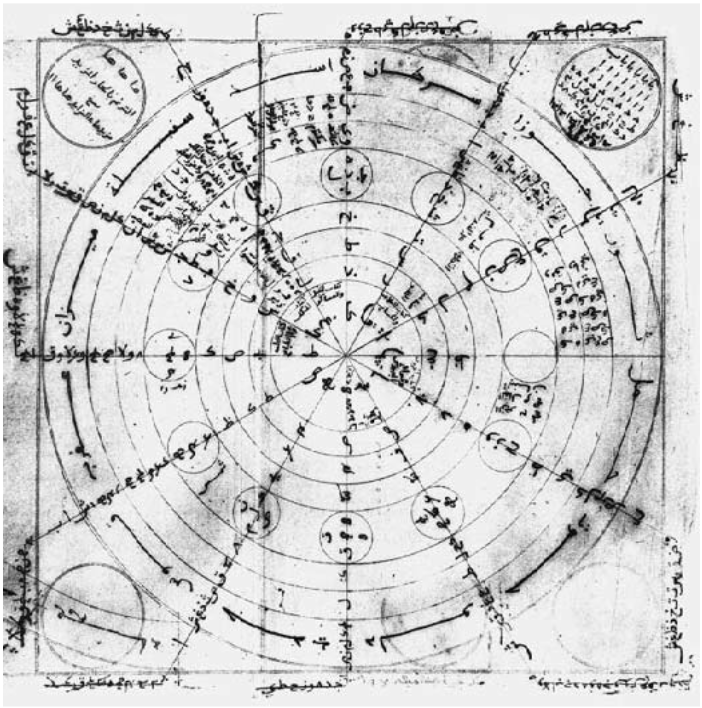
\includegraphics[width=0.49\textwidth]{ch1/images/zairja.png}
    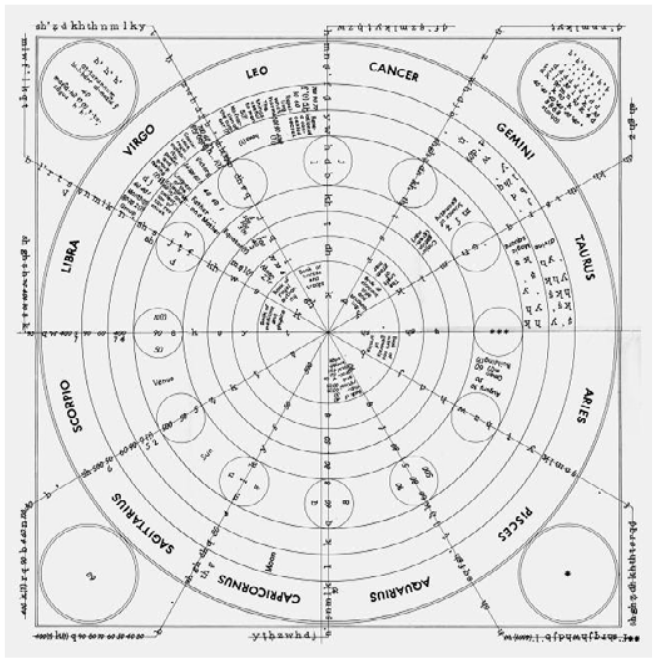
\includegraphics[width=0.49\textwidth]{ch1/images/zairjatl.png}
    
    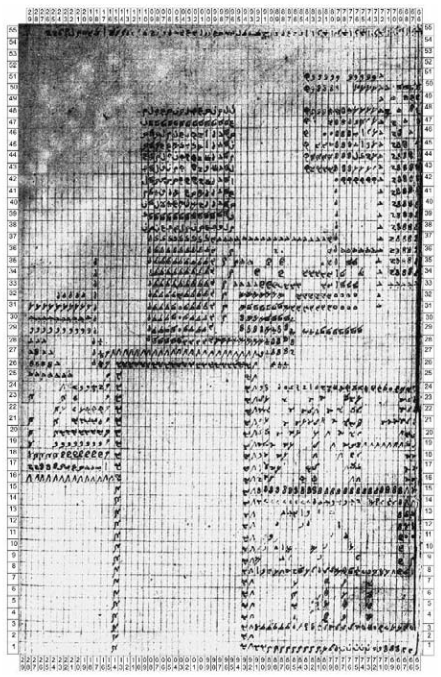
\includegraphics[width=0.6\textwidth,angle=90]{ch1/images/zairjaback.png}

    \caption{A zairja from a 15\textsuperscript{th} century Turkish manuscript of the \textit{Muqaddimah} \citep{link2010variantology}
        (top left), its transliteration from the English translation
    of \cite{rosenthal1958muqaddimah} (top right), and its lookup table (bottom).}
    \label{fig:zairja}
\end{figure}


{\color{red} Note to Kathy: the history of nlg sections are rough and I need to change them to reflect a new way of organizing the paper that I settled on so you can probably just skip ahead to section 1.4 on page 12.}

\section{A Brief History of NLG (antiquity-1950)}

The desire to build machines
that manipulate human languages is an old one. 
One early account of a language generation algorithm 
comes from 
14\textsuperscript{th} century historian 
`Abd ar-Rahm\={a}n ibn Khald\={u}n (1332 -- 1406), who
writes in the \textit{Muqaddimah} (1377) of a circular prognostication 
and divining tool  used by Sufi mystics called a \textit{z\={a}'irjah}.\footnote{Franz Rosenthal in his English translation of the  \textit{Muqaddimah} suggests the name is derived from 
the Persian words z\={a}'icha meaning ``horoscope'' or  ``astronomical table''
 and d\={a}'ira meaning ``circle.''}
 Its practice is
``a branch of the science of letter magic, practiced among the authorities on letter magic, is the technique of finding out answers from questions by means of connections existing between the letters of the expressions used in the question.'' 
Ibn Khald\={u}n points to an earlier treatise by the Sufi scholar 
Abu al-Abbas as-Sabti
(1129 -- 1204) of Marrakesh as a source of instructions for the device's use
\citep{rosenthal1958muqaddimah}, suggesting the practice is at least as
old at the 12\textsuperscript{th} century.

The \textit{z\={a}'irjah} itself consists of a series of concentric circles divided into 12 
sections by six chords. The various segments of the diagram are annotated with 
letters and numerals. Additionally, the \textit{z\={a}'irjah}  is accompanied by a lookup table mapping
letters to numbers. See \autoref{fig:zairja} for an example. According to painstaking reconstructions done by \citep{link2010variantology},
a ``key poem'' was used to pose a question to the \textit{z\={a}'irjah} and serve as a 
mnemonic device/mapping of letters to entries in the lookup table. 
A combination of rules and astronomical observations (the 12\textsuperscript{th} century equivalent of a random seed)
were then applied to the key poem to read off series of characters from
the \textit{z\={a}'irjah}. The operator
would then interpret those letters into an answer.  
``The fact that only consonants are written down in Semitic languages permits the meaningful interpretation of many random permutations of symbols,'' \citep{link2010variantology} suggesting that cherry-picking outputs and over-ascribing 
intelligence to a language generation algorithm are as old as the practice of
 NLG itself.

\begin{figure}
    \centering
    
\includegraphics[width=0.48\textwidth]{ch1/images/llull.png}
    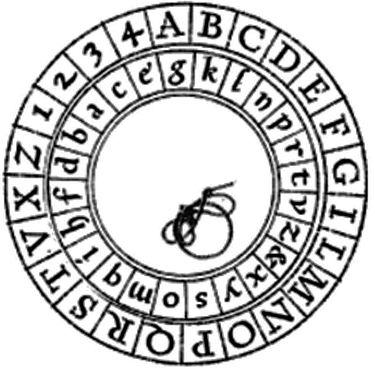
\includegraphics[width=0.48\textwidth]{ch1/images/cipher.JPG}
    \caption{(Left) A \textit{volvelle} from  Llull's \textit{Ars Magnus} 
    and (right) Alberti's cipher disk.}
    \label{fig:llull}
\end{figure}

\begin{figure}
    \centering
    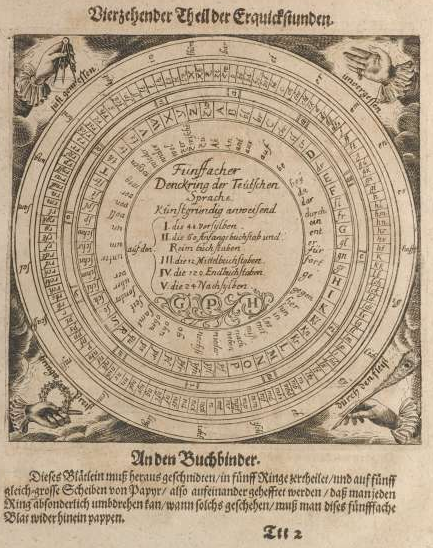
\includegraphics[width=0.98\textwidth]{ch1/images/baroqe.png}

    \caption{An illustration of the German word generator, \textit{F{\"u}nffacher Denckring der Teutschen Sprache}.}
    \label{fig:denckring}
\end{figure}



In a secondary account from a manuscript found at the library of Rabat, 
Morroco, it is written that a skeptical ibn Khald\={u}n asked of the device
how old it was: 
``[Is the] z\={a}'irjah [a] recent or [an] ancient science?'' 
and received the answer: ``The  Holy  Spirit  will  depart,  
its  secret  having
been brought forth / To Idr\={\i}s, and through it, 
he ascended the highest summit,'' drawing a connection to the sage
Idr\={\i}s who is one of the eldest
ancestors in the Quranic tradition \citep{rosenthal1958muqaddimah,link2010variantology}.



The teachings of Arabic mystics, including the practice of \textit{z\={a}'irjah}, as well 
as the Kabbalistic tradition embodied in the \textit{Sefer Yetzirah}
are known to have strongly influenced the 
Majorcan Christian mystic, Ramon Llull (1232-1315) \citep{kahn1980,sepllull,link2010variantology}.
%is known to have Arabic tradition  
%\textit{Z\={a}'irjah} are known to have influenced and similar practices from the Kabbalistic tradition 
%(the Sefer Yetzirah specifically) are known to have influenced the 
Llull, who is regarded as an early philosopher of combinatorics, logic, and 
computation \citep{sepllull,bonner2007art,knuth2013art}, developed 
a computational system based on moveable concetric circles made of paper
and connected by string. The workings of these \textit{volvelle}\footnote{The
    name \textit{volvelle} 
comes from the Latin, literally ``to turn''} are described in his master work,
\textit{Ars Magna} (1305). According to his system, concepts were assigned
letters which were manipulated to generate new knowledge and he claimed 
could be used to determine the truth of any proposition 
\citep{Crupi2019VolvellesOK}. Llull's work is also thought to have influenced 
the polyalphabetic substitution cipher developed by Leon Battista Alberti 
(1404 -- 1472) (see \autoref{fig:llull}), the same core cryptographic technology used 
in the Enigma machine  \citep{kahn1980}.


 \begin{figure}
    \center
    \noindent
    {%
        \setlength{\fboxsep}{0pt}%
        \setlength{\fboxrule}{1pt}%
        \fbox{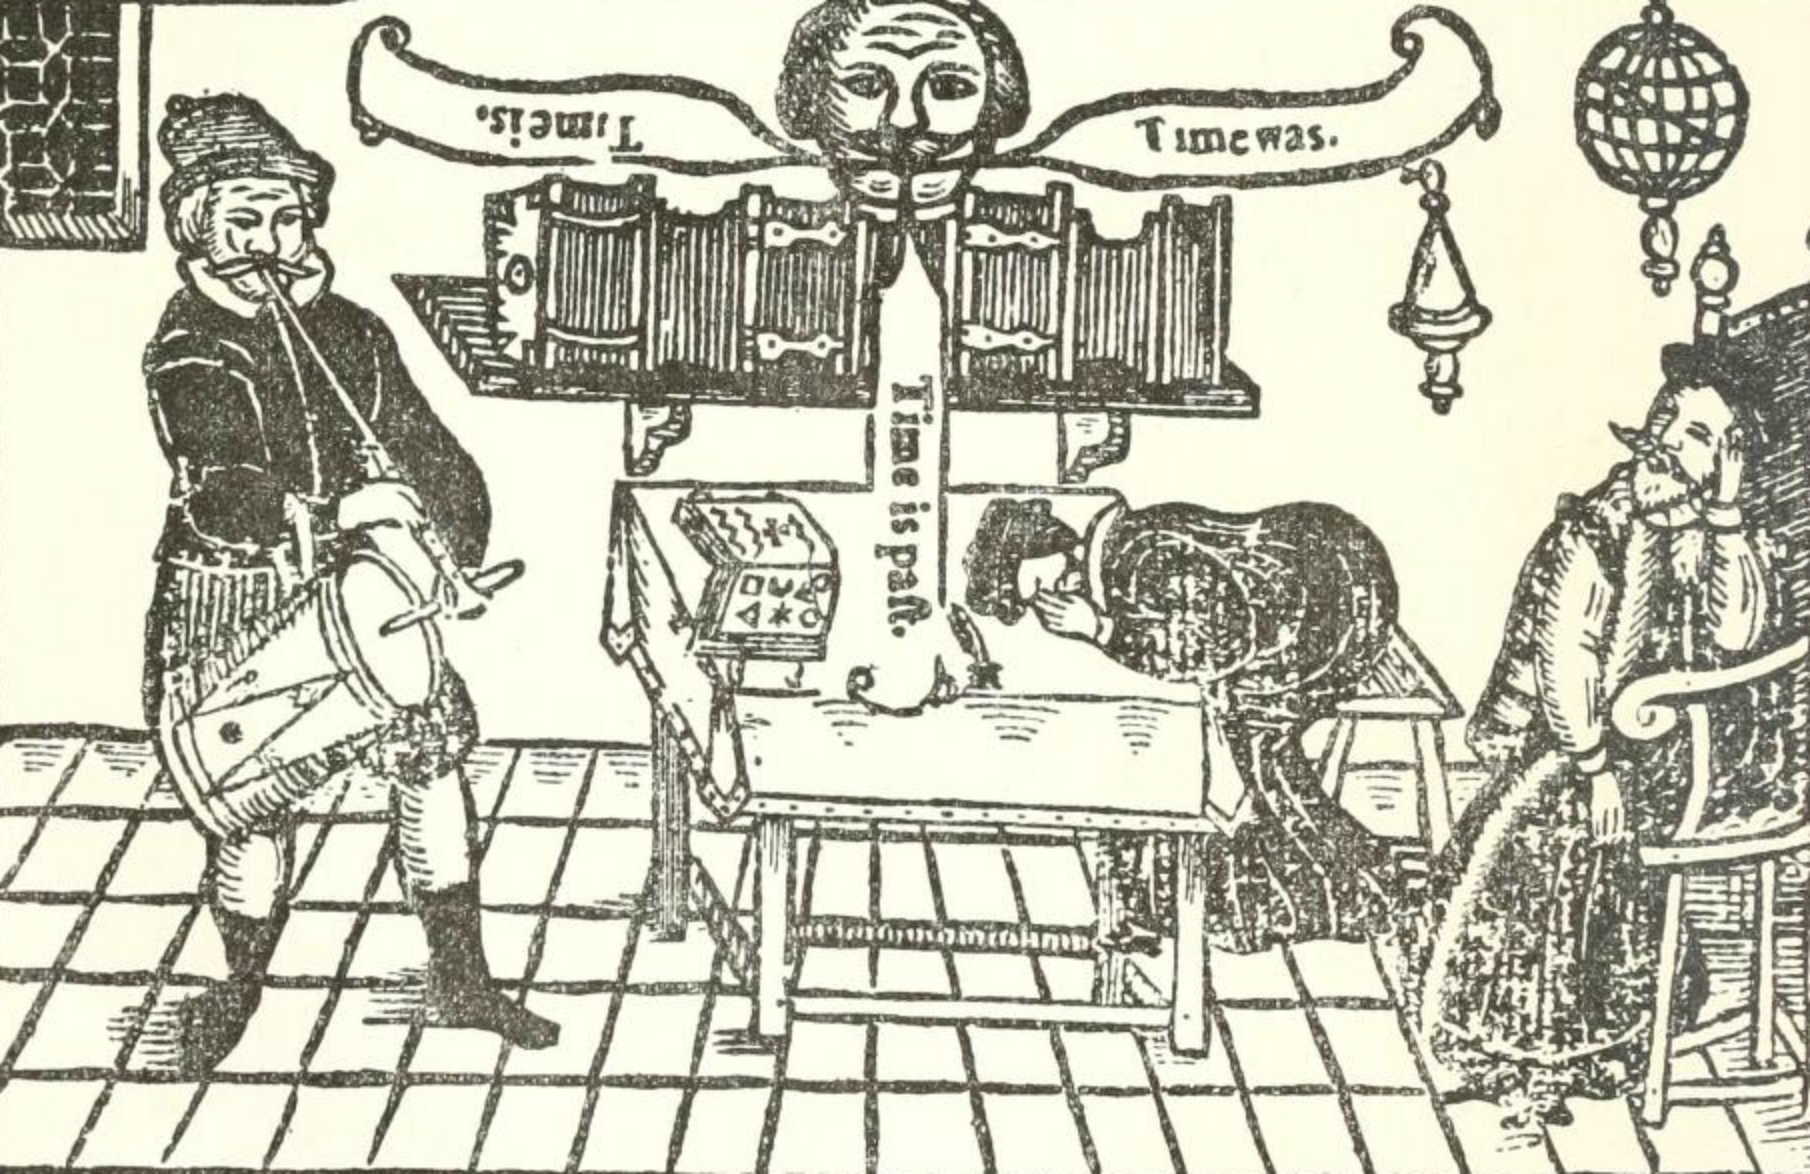
\includegraphics[width=0.7\textwidth]{brazen_head.png}}
}
\caption{A 1630 woodcut depicting Roger Bacon's talking bronze head, a mischievious talking autamata allegedly capable of answering any question \citep{hyman2016automaton}.}
\label{autamaton}
\end{figure}

\textit{Volvelle} were used throughout medieval Europe, arguably reaching
their zenith in the Baroque works of Georg Philipp Harsd{\"o}rffer (1607 -- 1658). His master work
\textit{volvelle},
\textit{F{\"u}nffacher Denckring der Teutschen Sprache} (1651), 
 consisted of five paper discs, and was claimed to faithfully model
 German word formation, and could aid in the production of poems and 
 other literary forms \citep{schafer2006literary}. See \autoref{fig:denckring}.



While computational devices before modern computing were limited in 
complexity by their construction
materials, chiefly paper, the dream of speaking automata was also
alive in myth.
See for example 
\autoref{autamaton}, in which a 17\textsuperscript{th} century woodcut print 
depicts a talking head capable of answering any question. This ``brazen head''
was allegedly built by the monk Roger Bacon, who in addition to being an
early philosopher of science and linguist, might also be considered 
the first natural
language processing (NLP) engineer if folklore is true \citep{sep-roger-bacon}.

%Depending on how loosely one defines an NLG algorithm, prayer, poem, and fortune generators have be found throughout many cultures in antiquity with
%prominent examples including volvelle \cite{} and lottery books \cite{}.
%Historical 
%evidence suggests these ideas were developed by Persian and Arabic scholars
%in the 9\textsuperscript{th}-??\textsuperscript{th} centuries \cite{},
%and eventually popularized in medieval Europe in the 13-1700s \cite{}. Volvelle
%are also notable for being used in early polyalphabetic substitution cyphers
% (the same core cryptographic technology used in the Enigma machine) \cite{}.


\section{A Brief History of NLG (1950-2010)}

Returning to the present day, computer aided 
production of human language closely follows the beginning of modern computing,
starting with work on machine translation (MT) systems developed 
in the 1950's and 60's \citep{ornstein1955mechanical,hutchins2003machine,national1966language}. Early work on producing extract summaries
of research articles also dates back to this period \citep{luhn1958automatic}.
There were also notable experiments in generating text purely from 
syntactic structures \citep{yngve1961random}.

However, NLG did not begin to coalesce as a distinct subfield until the 
1980s which saw
the first workshops devoted specifically to NLG  
and a convergence on the formalisms
and problems central to language generation \citep{reiter1997building,mcdonald2010natural}. 
NLG researchers of this period were focused on at least four
main research programs: (i) linguistically motivated grammars for generation,
(ii) frameworks for representating knowledge and concepts,
(iii) models of the human receiver of the generated text,
and (iv) models of discourse and control for planning the realization
of utterances \citep{mann1981text}. 


A variety of grammar and representation frameworks were proposed during this
period including Functional Grammar \citep{halliday2013halliday}, Transformational Grammar \citep{chomsky1965aspects}, Generalized Phrase Structure Grammar \citep{gazdar1985generalized}, \textit{et al.} and frameworks, including Knowledge
and Modalities Planner (KAMP) \citep{appelt1982planning}, Penman \citep{hovy1993natural}, MUMBLE \citep{McDonald1981MUMBLEAF}, TEXT \citep{mckeown1982text} and others \citep{mann1981text}.
While there appears to be a great diversity of approaches, most approaches
seem to converge on a fairly similar pipeline of modules when it came 
it implementation \citep{reiter1994has}. 

In particular, most NLG systems from this
period could be understood as a pipeline of modules for text planning,
sentence planning, and linguistic realization \citep{reiter1997building}.
In the text planning stage, the concepts to be conveyed are selected,
possibly discarding less essential information, and arranged into a discourse
plan or ordering. In the sentence planning stage,
the concepts from the previous stage are grouped into individual sentences,
and lexicalization of concepts and referring expression generation is performed.
Finally, in linguistic realization, the intermediate representation from 
the sentence planning stage is converted into a natural language utterance,
often by linearizing and inflecting some syntactic/morphological representation.

Since these systems primarily started from a non-linguistic representations 
of concepts, they are often referred to as 
\textbf{concept-to-text} generation or, as more commonly known today, 
\textbf{data-to-text} generation
\citep{gatt2018survey}. These systems were applied to a variety of data-to-text
problems including weather forecast generation \citep{goldberg1994using},
statistical report  generation (i.e. generating a report from numerical
or stastical data in a spreadsheet) \citep{iordanskaja-etal-1992-generation},
or as a writing aid to improve the productivity of human authors ().
Data-to-text generation came to prominence alongside expert systems \citep{todd1992introduction},
including as a means to explain them \citep{swartout1983xplain},
and often suffers from similar drawbacks. NLG systems often required extensive 
domain knowledge and manual rule or grammar engineering.

In the late 1990s and 2000s, as larger text corpora became available and statistical 
and/or machine learning techniques spread through the community, 
\textbf{text-to-text} generation (i.e. methods
of directly mapping unstructured text inputs to text outputs) increased in
popularity. Text-to-text generation is less defined by a specific 
generation task, method or unifying
theory, but on the use of large collections of example input/output text pairs.
For example, machine 
translation (MT), text simplification, and text summarization 
are all considered text-to-text generation when the approach uses
aligned sentence in input and output languages, pairs of complex and simple
sentences with similar meaning, and document/summary pairs respectively.


Some graph summarization  stuff.

Work on supervised learning for summarization begins to emerge from this
time \citep{kupiec1995trainable,osborne2002using,hirao2002extracting}. In these data-driven approaches, summarization
is framed as a sentence classification task, i.e. which sentences from the
input document should be included in a summary. While significantly constrained
in their expressive quality (i.e. only sentences found in the input can be
used to construct the output) especially compared to earlier data-to-text methods, designing features and focusing on the learning algorithm for performing
the generation task proved to be much more scalable. 
The Document Understanding Conferences start in this time, bringing together 
NLP researchers, particularly around multi-document summarization \cite{duc}.

The ability to generate more interesting or novel text also gradually increased
with time. In the unsupervised case sentence fusion \cite{fusion};
in the supervised case, learning syntax guided compression and extraction
appeared \cite{} although generation was still dificult and abstractive summarization was rare \cite{maybemckeownnenkova}.



\section{A brief history of NLG (2010-present)}

While neural networks had been used previously as part of phrased-based 
statistcal MT (SMT) systems \cite{}, there was an increased interest in
the early-mid 2010's around using recurrent neural network (RNN) language 
models \citep{miklov}
as a rescoring method for an SMT decoder \citep{auli2013joint,cho2014learning}.
While previous approaches 
used feed-forward networks, RNNs could exploit (in theory) unbounded source
and target prefix information that was difficult to caputre in n-gram or 
feed-forward models. \citet{cho2014learning} is particularly noteable because
they propose separate encoder/decoder RNNs, and while intended for rescoring
and not generation directly, this general architecture 
constitutes ``sequence-to-sequence'' backbone of most neural MT (NMT) and 
neural NLG models.

Shortly thereafter, \citet{sutskever2014sequence} proposed the now ubiquitous 
sequence-to-sequence model to perform translation directly. \citet{bahdanau2015neural} (2014 on arxiv) also propsed a sequence-to-sequence model with 
an attention mechanism, which both made optimization easier, (error feedback,
 i.e. gradients, could now be routed directly from any decoder word prediction 
 step to
 any arbitrarily  distant timesteps in the encoder)
 and allowed for visualization of NMT decoder's alignment with the encoder
 (see \autoref{fig:nmtattn}).
NMT models, while conceptually simpler than phrase-based SMT, were starting
to achieve state-of-the-art results \cite{} and wide-spread industry adoption
\cite{wu2016google}.

It did not take long for researchers to adapt the sequence-to-seqeunce model
to other language generation problems, e.g. generating captions from images \cite{},
sports summaries for box scores \cite{}, or, echoing the dreams of 80s NLG, 
from semantic representations \cite{}. In summarization, sequence-to-sequence
models were quickly adapted to generate headlines and eventually full summaries\cite{}, and copy-mechanisms were developed to blur the extractive/abstractive
summarization distinction \citep{}. Given parallel object/text pairs,
it now became increasingly easy to develop a plausible conditional NLG system,
while far from perfect \cite{}, it is hard to under-estimate effects
of the deep learning paradigm on language generation.

In \citeyear{vaswani2017attention}, \citeauthor{vaswani2017attention}
proposed a recurrence-free neural sequence model, built around so-called 
\textit{transformer} layers,
which rely on mulitiple parallel self and context attention mechanisms.
This model was designed with optimization speed in mind, and was subsequently
used in large scale language modeling pretraining on web-scale text, 
spawning the BERT-family
of models \citep{}. BERT has since been used as a non-autoregressive means
of generating text \citep{}. 

The transformer layer was also used in the (generative pre-training) GPT
family of models \citep{}, which also trained on web data, but with an
auto-regressive language modeling objective. The second generation of 
these models, GPT-2, reveived notoriety both amongst NLP researchers but 
also the wider public, as it's release was initially delayed given ``ethical
concerns'' about releasing such a powerful language generation model \citep{}.
Regardless of the merits of these claims, the model was eventually released
and does exhibit impressive prefix capabilities, generating longer spans
of fluent text than previously thought possible. 

Like BERT, GPT-2 could used in a fine-tuning setting, and used in a 
variety of conditional generation settings \citep{}. BART \citep{bart} and
T5 \cite{t5} followed with sequence-to-sequence variants of the 
large transformer-based model pretrained on denoising autoencoder and 
other pretraining objectives, where both models are designed to be fine-tuned
on sequence-to-sequence language generation tasks. 


\section{Problems in Text-to-Text Generation}

As envinced by this brisk journey through the history of \languagegeneration,
\machinelearning~has emerged as the \latin{de facto} methodology for 
solving both \texttotext~and~\datatotext~problems. \Deeplearning~models in 
particular have shown themselves to be both versatile and empirically 
successful solutions. However, the inner workings of such models are often 
opaque and difficult to 
control or understand in practice. In this thesis, we offer modeling 
methodologies to establish control or understanding in a variety of  
\machinelearning-based models of summarization. At a high level, the 
first two chapters focus on \contentselection.
The last chapter focuses on \surfacerealization, that is, generating text
from an idealized representation of the content selection stage. 
%in the idealized case of problems, effectively focusing
%on the actual language generation component, i.e. how to say it. (note to self, cite Kathy's work here).

In this section, we will briefly introduce the tasks and problems that will 
ground the experiments and analyses of this work. More formal definitions
can be found in the individual chapters. 
%It is for this reason that we focus on extractive summarization in this work.
%\Automaticsummarization~as it is studied in the 
%\naturallanguageprocessing~literature typically dichotomizes summarization
%approaches into either \extractive~versus \abstractive~methods \cite{something}. 
%In the former case, a summary is constructed by essentially copying and 
%pasting the input utterances to obtain a summary; in the latter case, the 
%summary content is generated from scratch, synthesizing the input content in
%some manner to produce the summary. In practice, systems are often composed of
%a mixture of extractive and abstractive techniques, e.g., using sentence 
%compression on top of extraction. We study the extractive task since it allows
%us to focus on the salience estimation task directly, while not having to
%implement an abstractive generation component (which is typically more
%computation and memory intensive than, and more difficult to evaluate). 
%
%
%
In most summarization problems, we are generally interested inf 
a text's \textit{\salience}, that is to say, the general importance or relevance of 
a given text unit with respect to its context. \Salience~is usually the primary dimension of the input data that we wish to 
measure or predict for summarization problems. 
In \autoref{dlsal}, we study \salienceestimation~in 
the \emph{sentence extractive, single document summarization task}, 
where the goal is to classify which sentences in an input document should be 
included in an extract summary. 
In this case, the input document is the context, and the units of text for 
which we are estimating salience are the document
sentences. An extractive summary is a subset of sentences that have maximum
salience while sastifing a length budget constraint, typically in the summary
word or byte length. While the constrained subset selection problem is 
interesting and has been studied previously \cite{maybemmr,mcdonald,others},
we focus on modeling the salience estimation task specifically. 

%?Since salience is not usually explicitly available in most summarization 
%?datasets, we approximate it by first constructing an extract summary from input
%?document the greedily maximizes a measure of ngram overlap with a human
%?reference abstractive summary subject to the length constraints. We then
%?consider as salient those sentences which were select for the extract 
%?summary.

We study a variety of popular and novel \deeplearning~architectures for 
implementing the salience prediction task. Our key contribution here is not
a modeling architecture, but our systematic study of the combination of 
sentence and context (i.e. document) level encoders as well as the 
manipulation of the input documents to ablate which surface features are 
available to a given model. Through these input data ablations, we can gain
a better understanding of how the salience prediction mechanism is working.


In \autoref{mlsal}, we study a more difficult summarization task, 
\emph{query focused, streaming, sentence extractive summarization}. In this
task, we add a search query and time as additional elements to the 
summarization problem. As input we are given a time-ordered stream of news 
articles and a query, typically an notable real-world event, 
e.g., \texttt{``Hurricane Sandy''}. Our objective is to extract sentences that
are relevant to the query event while minimally redundant to previously 
extracted
sentences. Unlike the previous problem, the salience of given sentence 
is not constant but monotonically decreases as time goes on. In addition
to modeling the salience, we must now also model the redundancy between
sentences. 

The main contributions of this work are to show that with careful feature 
design, we can capture salience beyond using the position-based heuristics
that we found the neural models to use. In particular, we show that content
based, time, location, and redundancy features can be used to predict salience
in this more challenging scenario.

We encorporate these features into two possible approaches for streaming
summarization.
The first method works in time ordered batches, processing all sentences that 
occur in \autoref{times}-hour windows of the news the stream. The actual summarization method happens in two stages. In the first stage salience of the individual
sentences is estimated. Then, those salience predictions are used to bias
an exemplar base clustering algorithm, such that the cluster centers are both
representative of cluster members but also highly salient. 


The second method works by making sequential prediction on sentences from 
the input news stream immediately, without batching or waiting to collect 
a reservoir of a certain size. This model employs a learning-to-search style
of algorithm \cite{searnorlosl} to avoid exposure bias inherent to these
extended sequence prediction tasks.


In \autoref{gen}, we move to problems of \surfacerealization~after the content
selection process has been performed. 
Here we focus on the related goals of
\term{faithful}~and~\term{controllable}~generation. A faithful language 
generation model generates utterances that are semantically correct
with respect to the information extracted in the 
content selection stage.
%a reframing of the evaluation of \naturallanguagegeneration~from fluency and
%to semantic correctness 
Controllable generation models represent a subset of 
faithful generation models. Controllable generation models follow
an explicit plan that guides the surface realization order of the generated utterance.
Faithful but uncontrollable models will generate semantically correct 
utterances but the decoder language model implicitly controlls the surface
realization order by generating the next utterance word.

Evaluating the faithfulness of a language generation model for open-world
summary generation tasks is non-trivial. In order to simplify things,
we study faithful and controllable generation in the context of 
\emph{\taskorienteddialoggeneration}, 
 where given an explicit representation
of a dialog agent's belief state and goals, we must generate an appropiate
natural language utterance. Because the input is an explicit, formalized 
representation of the meaning of the intended utterance, manual and 
even automatic checking of the faithfulness of an
utterance/meaning representation pair becomes much simpler. Since the concerns
of faithful and controllable generation are still relevant to generating
summaries, we consider the explicit meaning representations as 
an idealized version of summarization system's content selection stage.


%In \taskorienteddialoggeneration, the dialog agent
%has a communicative goal that it is trying to achieve. Crucially,
%the input to the agent is an explicit representation of the meaning 
%of intended utterance.
%
%
%In \autoref{gen}, we move to the \datatotext~problem of 
%\emph{\taskorienteddialoggeneration}, where given an explicit representation
%of a dialog agent's belief state and goals, we must generate an appropiate
%natural language utterance. In \taskorienteddialoggeneration, the dialog agent
%usually has a goal that they need to achieve. For example, a dialog agent may
%want to book a reserveration at a restaurant but inorder to do that, it 
%needs to ask a user for a range of possible times that are acceptable to
%place the reservation. In this case, input to the dialog generation 
%component would be a representation describing a \texttt{request information} dialog act, with the desired missing information explicitly represented,\texttt{reservation time range}.
%
%When deep learning models are used to generate text in scenarios like these,
%they are usually effective at generating fluent and natural text \cite{}.
%However, without careful treatment, the frequently generate utterances
%that do not accurate reflect the input meaning representation. In the
%case above for example, they might accidentally request the  location 
%instead of the time. 


For our contribution to faithful generation, we propose a novel 
data augmentation method that uses an unfaithful NLG model and an NLU model 
to generate novel and semantically diverse utterance/meaning representation 
pairs that can be used as additional training data. Sequence-to-sequence
models trained on the union of original training data and the synthetically
generated training examples exhibit increased faithfulness.

% to remove spurious correlations from the 
%training data and obtain a 
%neural \naturallanguagegeneration~model with reduced semantic errors.

While this data augmentaiton method helps reduce semantic errors, it leaves the surface
realization of utterances up to the decoder language model. In \autoref{gen}
we also investigate an encoder input transformation, applicable to arbitrary \sequencetosequence~models, that reliably results in a controllable generation 
model. 


%
%it occurs in)
%
%We start in the single document extractive summarization case, 
%where the task is 
%to predict a subset of an article's sentence to include in a summary.
%We explore several popular neural architectures for performing this 
%task and systemaically evaluate them under different noisy input ablations.
%These ablations allow us to isolate different features of the input.
%
%
%In the second chapter, we explore two classical machine learning models
%applied to the harder problem of query focused extractive stream summarization. 
%In this setting we propose two models, one that 

\section{Contributions}

We now briefly summarize the contributions of this thesis described
in the previous sections.

%This thesis  makes the following contributions to NLG.
%In the areas of text-to-text generation,

\begin{enumerate}
        \item We propose a systematic evaluation of deep learning models
            for extractive single document summarizations (\autoref{}). 
            Our evaluation on several popular neural architectures shows 
            that:
            \begin{itemize}
                \item Position features, even when not explicitly represented
                    in the model architecture are a dominant feature
                    exploited by the model.
                \item Content features exist across a variet of word classes
                    but are not as strong of a signal as position.
                \item Word embedding averaging is about as effective as 
                    recurrent or convolutional sentence encoders 
            \end{itemize}
        \item Additionally, in the task of query focused streaming news 
            summarization, we propose two models for providing 
            extractive update summaries. (\autoref{})
            \begin{itemize}

                \item The first method processes the stream in  batches. 
                    It uses a regression model
                    to estimate the salience of individual 
                    sentences, and a biased clustering algorithm to select
                    the most representative and salient outputs.
                \item The second method processes the stream in a fully
                    online manner. A linear model makes extraction
                    decisions, and we experiment with a learning-to-search
                    algorithm for training. 
            \end{itemize}
    \end{enumerate}

    In the area of data-to-text generation, we make the following 
    contributions to faithful and controllable generation of 
    text from a meaning representation. 
    \begin{enumerate}
        \item We propose a noise injection and self-training method
            for obtaining a faithful NLG model.
        \item We propose an encoder input linearization called alignment
            training which  yields an NLG model with surface level
            realisation ordering control.
    \end{enumerate}


Finally, in chapter \autoref{conc} we conclude with a discussion of the 
limitations and future 
directions this work might take. In particular, we focus on how 
faithful generation might be applied to summarization or \machinetranslation
where an explicit representation of the content meaning is not available. 





